\section{Description and methodology}

The exercise as a whole was done as suggested in the compendium, by starting with implementing the solution to exercise 1 in C and learning to use the debugger for debugging C-code, then doing the DAC part. 
We started the sound part by making sure the hardware was working with just outputing noise from the C \texttt{rand()} function, then moved on to playing sine and square tones.
Finally we made code for playing and recording (saving) songs.

\subsection{Sound}
For the sound effects, we chose to use sine waves rather than square or triangle waves for a more 'organic' feel to the sound. We used a C program to generate (sample) the different tones in advance and saving them as arrays in the header file for quick lookup, at the expense of memory.
The songs are comprised of lists of notes. A note is made by saving indices into an array of all the presaved tones, giving the tone, together with a value for how many samples the tone consists of and for how long - how many interrupts - to hold the tone. 
This is enough to allow for entering songs in a somewhat musical fashion. We keep a global pointer to a \texttt{Song} struct, which points to the song currently being played. We also hold pointers to the sample currently in use, and counters to remember where in the sample we are, how long the tone has been playing and for how long we are supposed to play it.
When a song is done playing, we switch off the DAC until a new song is loaded by calling the \texttt{playSong()} routine. This routine sets up the nescessary pointers and indices to start playing the \texttt{Song} given as argument, in addition to enabling the DAC, clock and interrupts.
%insert figure of sampling a sine wave
%\begin{figure}[here]
% \includegraphics{img/sinewave.png}
% \caption{Sampling of a sine wave. The amplitude is saved at certain intervals and recreated in the digital-to-analog converter by entering (outputing) the saved amplitudes at the same intervals.}
% \label{fig:sinewave}
%\end{figure}
\subsection{Overall hardware setup}

All jumpers were set as specified in the exercise description. We also chose to use the internal DAC.
PIOB pins 0-7 was connected to the 8 buttons, while pins 0-7 on PIOC was connected to the leds.
We also had to disable pins 20 and 21 from being driven by the GPIO, so they could be used by the internal DAC, as specified in the compendium.

\subsection{IO controllers}
The different controllers on the STK1000 mostly have structs defined in the avr32 code that can be used to simplify interfacing with them. This is done by having a struct, e.g. the \texttt{avr32\_pio\_t} represent the memory structure around the IO controllers PIOB or PIOC. 
Making this struct point to the base address of the IO controller, allows for simple access to the different registers in the controller, which are accessed through fixed memory addresses and offsets. 
In example, turning off output on IO pins 0-7 on PIOB, can be done by executing \texttt{piob->CODR = 0xff}, given that piob is a pointer of type \texttt{avr32\_pio\_t}, and pointing to the base address for the PIOB IO controller.
The abdac and power manager also have similar structures for control in the datatypes \texttt{avr32\_abdac\_t} and \texttt{avr32\_pm\_t}, respectively. 
It is also important to note that these variables should be declared as volatile to avoid potential bugs introduced by compiler optimizations.

\subsection{Controlling the LEDs}

With our setup the 8 LEDs can be controlled through PIO port B pins 0 - 7. We started by enabling these pins on the IO-controller. This is done by writing 0b11111111 to the address for PIOB + offset for the enable register (called PIO\_PER). Next we enabled output on the pins by writing 0b11111111 to the address for PIOB + offset for the enable output register (called PIO\_OER). Which LEDs are actually turned on can be controlled by writing to the register with offset PIO\_SODR, and turned off by writing to the register with offset PIO\_CODR, together with an 8-bit bitmask corresponding to LED 0-7.

\subsection{Interrupts}

Interrupts were set up with the use of the functions specified in the \texttt{interrupts.h} header file. A call to \texttt{register\_interrupt} takes 4 arguments: 
a function which is called when the interrupt goes off, the interrupt group and line, and the priority this interrupt is to be assigned. \texttt{set\_interrupts\_base} and \texttt{init\_interrupts} takes care of the system wide setup of interrupts in general, like the GM bit and EVBA, which both must be set.

\subsubsection{Buttons}
The button interrupts are handled by the \texttt{button\_isr} routine, and is registered with the earlier mentioned \texttt{register\_interrupt} routine. The \texttt{button\_isr} routine starts with reading which button caused the interrupt, then checks if this button is actually pressed down and not being released. If the button is being released, the interrupt routine returns.
Each button has a designated function. The first and last buttons move the LED light one step to the right or left, respectively.
The buttons inbetween sets the LED light to the same as the button being pressed, and starts playing a sound or melody if this functionality is set up.

\subsubsection{ABDAC}
The internal DAC interrupt handling is also set up by calling the \texttt{register\_interrupt} routine, which makes sure the \texttt{abdac\_isr} routine is called on every interrupt from this device.
% TODO: figure out exact freq of oscillator 0 so we know what freq we are sampling for
The interrupts are done by a clock (oscillator) polling the abdac with a frequency of 12 MHz, with the abdac only asserting the interrupt line on every 256th clock pulse. 
This gives the DAC a sampling frequency of about ~46 kHz.
On every interrupt, the offset to the next sample 


\subsubsection{}


%%%%% Here and down is from last exercise.
%%%%% 
%%%%% 
%%%%% kept around for inspirational reasons
%%%%%
%%%%%
%%%%% 
The AVR32 supports interrupt driven IO. To enable interrupts on our buttons several things must be taken care of. First we need to tell the IO-controller to enable interrupts on the buttons. This is done by writing to register with address PIOC + offset PIO\_IER. Next the interrupt controller needs to get an address (14 bits) in the register corresponding to interrupts from PIO\_C on line 0. The code at this address is the interrupt routine code that will be called. This address is called the autovector. The full address for the code called however, is the result of the variable EVBA + the autovector. In this exercise we can set the EVBA to 0 and just pass the address for where our interrupt routine resides, which helps simplify. Lastly we must enable interrupts for the whole system by setting the GM bit, done by the instruction \texttt{csrf 16}.



\subsection{Main program}
%\pagebreak
\begin{figure}[here]
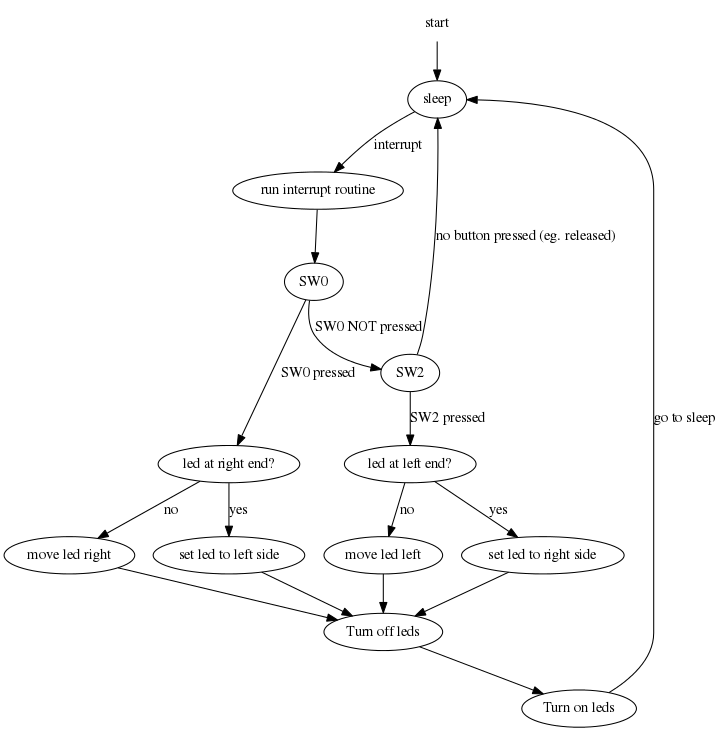
\includegraphics[width=0.9\textwidth]{img/graph.png}
\caption{Flowchart showing the flow of the main program loop and the interrupt routine. Notice the button precedence.}
\label{fig:mainflow}
\end{figure}

\begin{table}
 \centering
 \begin{tabular}{| c | l |}
    \hline
    \textsc{CPU Register} & \textsc{Contains} \\ \hline
    \texttt{r0} &       Address for PIO port B \texttt{PIOB}. \\
    \texttt{r1} &       Address for PIO port C \texttt{PIOC}. \\
    \texttt{r2} &       Address for interrupt controller \texttt{INTC}. \\
    \texttt{r7} &	Bitmask for enabled LEDs (lower most 8 bits) \\
    \hline
 \end{tabular}
 \caption{CPU registers used}
 \label{table:cpuregs}
\end{table}

The main program is a loop structured as the flowchart of Figure \ref{fig:mainflow}. We start off however by loading the addresses of PIOB, PIOC and the IO controller into registers r0, r1 and r2, respectively (not shown in figure). We then continue to set up the different io controllers and cpu as described in the sections above. The autovector is set to the address of the \texttt{handle\_interrupt} routine. The routine first determines if one of our predetermined buttons caused the interrupt, then figures out which one of these buttons is pressed right now, if any. If the correct button is pressed during the interrupt, the program then does a logical right or left shift of the LED lights, according to the button that was pressed. If the result after the logical shift is too big, or too small, the LEDs are reset to light up on the other end. E.g. if the value of the enabled LEDs is 0 after a logical right shift, it means that we should reset the light to show up on the other side. This works similarly for the left to right button, where we check if the value is bigger than the 8 lower bits. We then clear all the glowing LEDs and enable the row with the new bitmask, \texttt{rete} (return from interrupt) and go to sleep again. An overview of CPU registers in particular use is given in Table \ref{table:cpuregs}.


